\section{Pebble Damage Modeling}\label{sec:failure-study}
% \cite{Hiramatsu1966}
% From , 
% \begin{align*}
% \sigma_{cr} = \cfrac{2.8}{\pi}\cfrac{F_{cr}}{4R^2}
% \end{align*}
Research on pebble damage has been taken up by others in the fusion community to predict the onset of pebble crushing as a function of an external pressure and the resulting changes to mechanical properties such as the stress-strain of the pebble bed.\cite{Annabattula2012a, Zhao2012, Zhao2013} Other fields of engineering have also employed DEM in studies of granular crushing with generally similar modeling approaches.\cite{Marketos2007,Pitchumani2004}


In modeling pebble damage, there are two main tasks: predicting when the grain crushes and what happens when it does. For the former, the task is to develop a model for predicting a pebble crushing event; \textit{i.e.} what load (mechanical or thermal) will cause a pebble to crack, shatter, fracture, etc. To tackle the latter is to develop a model which simulates the damage of that pebble; \textit{i.e.} a scheme to treat a cracked, shattered, or crushed pebble in the assembly as small particles, removed particles, or particles with modified material properties.

\begin{figure}[!t]
\centering
	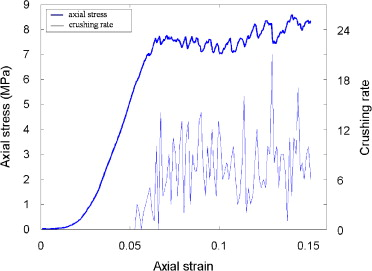
\includegraphics[]{chapters/figures/markets-bolton-stress-strain-crushing.jpg}
	\caption{Stress-strain response of a pebble bed with crushed pebbles. Reproduced from Ref.~\cite{Marketos2007}}
	\label{fig:marketos-bolton-stress-strain}
\end{figure}

\begin{figure}[!t]
\centering
	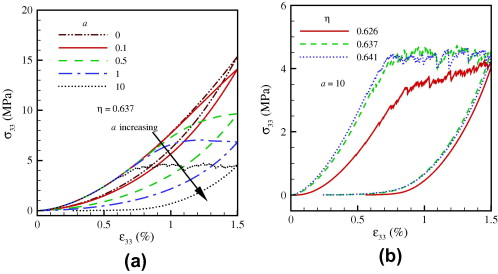
\includegraphics[]{chapters/figures/annabattula-stress-strain-crushing.jpg}
	\caption{Stress-strain response of a pebble bed with crushed pebbles. Reproduced from Ref.~\cite{Annabattula2012a}}
	\label{fig:annabattula-stress-strain}
\end{figure}

This numerical study will focus on the `what happens' question. In work by Marketos and Bolton, they treated a crushed pebble very similar to Van Lew\etal~; when a pebble was damaged it was removed completely from the assembly.\cite{Marketos2007,VanLew2014} Marketos and Bolton study the stress-strain response of a pebble bed with a predictive crushing routine while we studied the effective thermal conductivity of a damaged pebble bed.

However, the technique of removing a pebble is limited by the fact that energy input into two systems being studied is not comparable. Because we have volumetric energy deposition in our simulations, the total energy pouring into the non-damaged system would be
\begin{equation}
	E_h = \frac{q'''_\text{nuc} V_\text{peb} N}{V_\text{bed}}
\end{equation}
where $N$ is the total number of pebbles of volume $V_\text{peb}$ that exist in the pebble bed of volume $V_\text{bed}$. After a crushing event, when we remove pebbles, the total amount of energy is
\begin{equation}
	E_h' = \frac{q'''_\text{nuc} V_\text{peb} \eta N}{V_\text{bed}}
\end{equation}
where $\eta$ is the percent of crushed pebbles. Obviously then, the ratio of the two heating rates is\begin{equation}
	\frac{E_h'}{E_h} = 1 - \eta
\end{equation}
and the energy deposited is not balanced between a virgin bed and one with crushed pebbles. We will attempt to address this issue.

\subsection{Modeling a Crushed Pebble}
In the DEM framework, we are limited to modeling elastic spheres. If we strictly wish to conserve mass between a solid pebble of radius $R_p$ and the crushed fragments of radius $R_c$, then the number of crushed fragments (spheres) per crushed pebble is
\begin{equation}
	N_c = \left(\frac{R_c}{R_p}\right)^{-3}
\end{equation}

Thus the number of fragments goes like the inverse of radius ratio to the third power and the number of crushed fragments to represent a single crushed pebble increases rapidly as the fragments shrink.


\begin {table}[htp] %
\caption{The particle crush fragments, $N_c$, necessary to replace a single crushed particle and obey conservation of mass.}
\label {tab:rstar-Nc} \centering %
\begin {tabular}{ cc }
\toprule
$R_c/R_p$ 						& $N_c$  				\\\otoprule
0.2                             & 125                   \\    
0.25                            & 64                      \\  
0.3                             & 37.0               \\
0.35                            & 23.3               \\
0.4                             & 15.6                    \\
0.45                            & 11.0                \\
0.5                             & 8                         \\
0.75                            & 2.4                \\\bottomrule
\end{tabular}
\end{table}






\begin{figure}[!ht]
	\centering
	\begin{subfigure}[b]{\imagewidth}
		\centering
		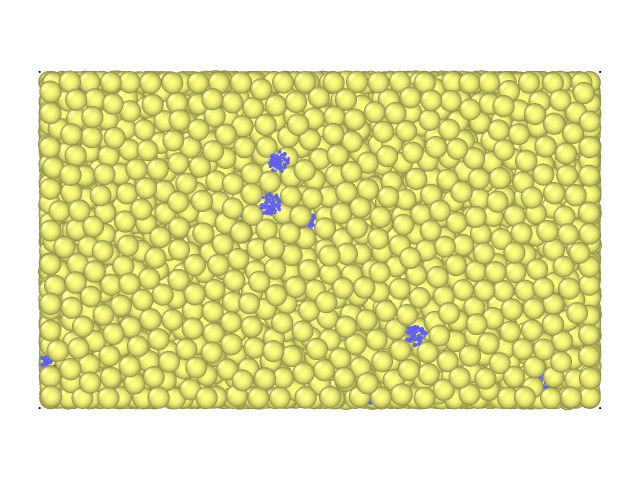
\includegraphics[width=\textwidth]{chapters/figures/crush-fragments/0.20-1.png}
		\caption{$R^* = 0.20$, initial}
	\end{subfigure}
	\begin{subfigure}[b]{\imagewidth}
		\centering
		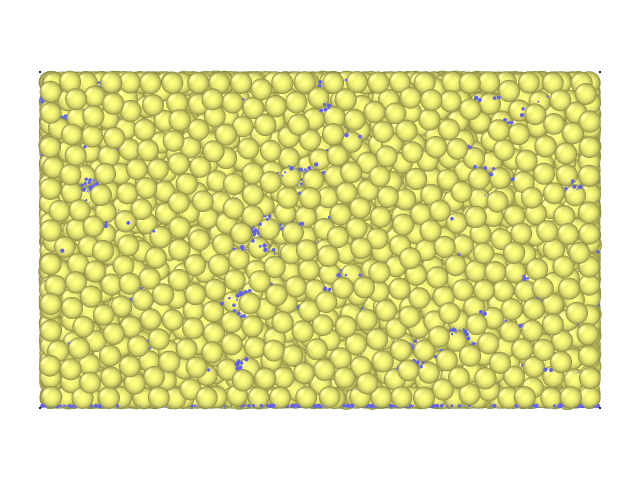
\includegraphics[width=\textwidth]{chapters/figures/crush-fragments/0.20-2.png}
		\caption{$R^* = 0.20$, final}
	\end{subfigure}
	
	\begin{subfigure}[b]{\imagewidth}
		\centering
		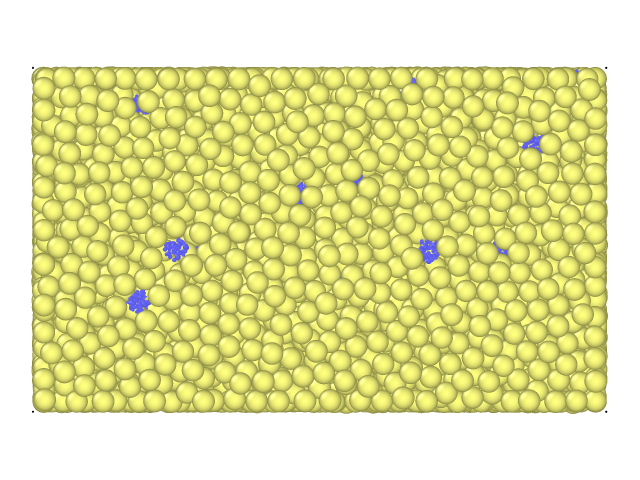
\includegraphics[width=\textwidth]{chapters/figures/crush-fragments/0.25-1.png}
		\caption{$R^* = 0.25$, initial}
	\end{subfigure}
	\begin{subfigure}[b]{\imagewidth}
		\centering
		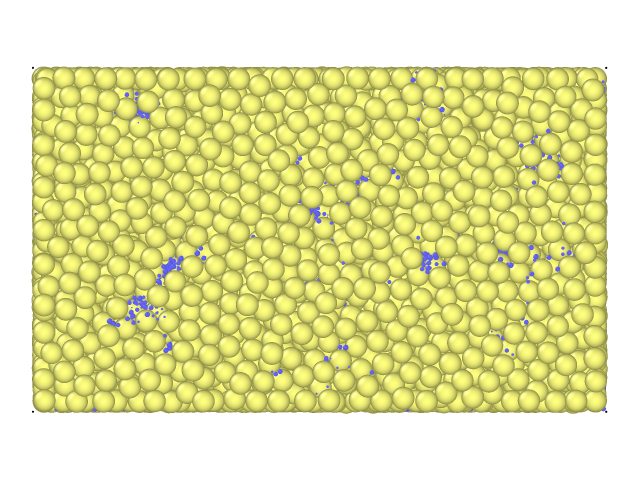
\includegraphics[width=\textwidth]{chapters/figures/crush-fragments/0.25-2.png}
		\caption{$R^* = 0.25$, final}
	\end{subfigure}
	\caption{The packing arrangement and settling for different crush fragment sizes. The small crush fragments migrate far through the height of the bed.}
\label{fig:crush-settling-pictures-1}
\end{figure}

\begin{figure}[!ht]
	\centering
	\begin{subfigure}[b]{\imagewidth}
		\centering
		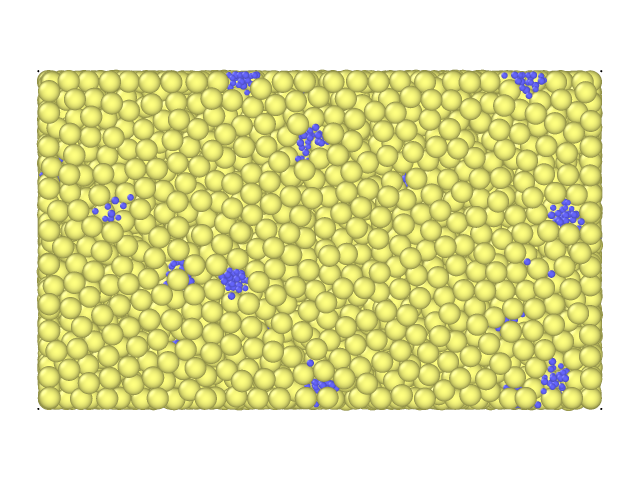
\includegraphics[width=\textwidth]{chapters/figures/crush-fragments/0.35-1.png}
		\caption{$R^* = 0.35$, initial}
	\end{subfigure}
	\begin{subfigure}[b]{\imagewidth}
		\centering
		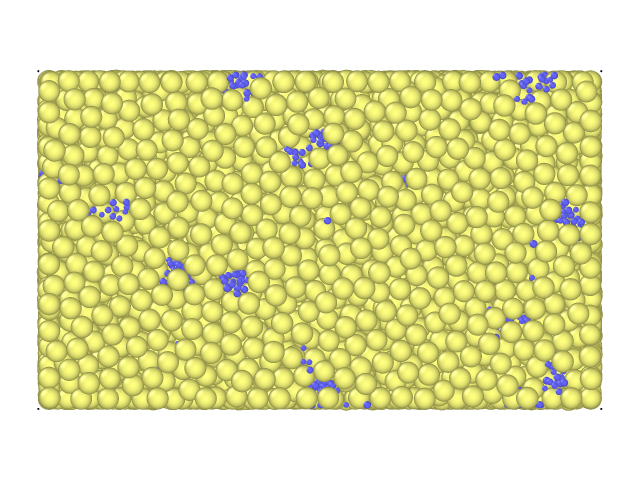
\includegraphics[width=\textwidth]{chapters/figures/crush-fragments/0.35-2.png}
		\caption{$R^* = 0.35$, final}
	\end{subfigure}

	\begin{subfigure}[b]{\imagewidth}
		\centering
		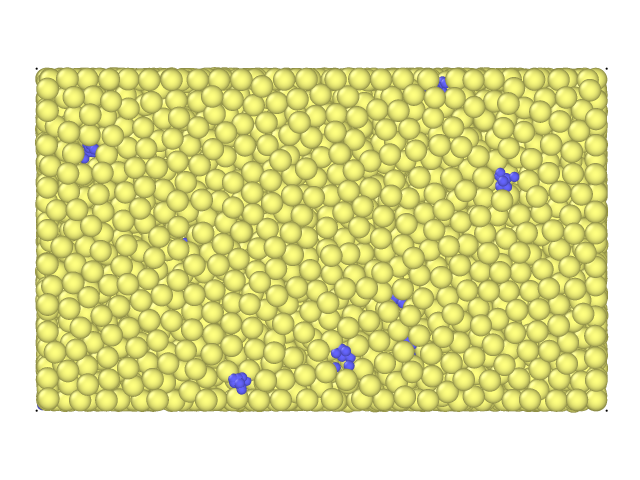
\includegraphics[width=\textwidth]{chapters/figures/crush-fragments/0.50-1.png}
		\caption{$R^* = 0.50$, initial}
	\end{subfigure}
	\begin{subfigure}[b]{\imagewidth}
		\centering
		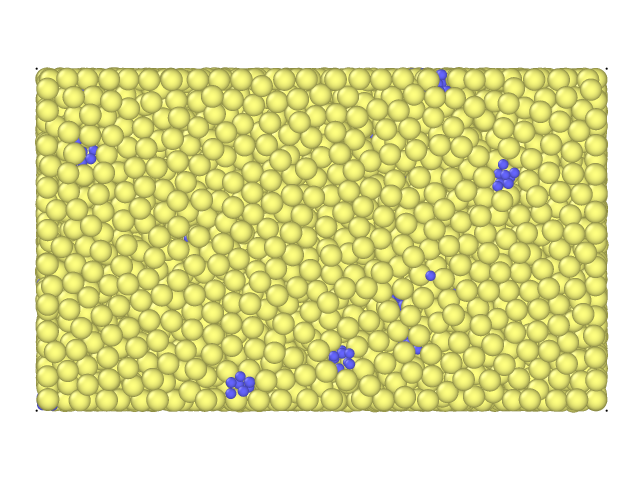
\includegraphics[width=\textwidth]{chapters/figures/crush-fragments/0.50-2.png}
		\caption{$R^* = 0.50$, final}
	\end{subfigure}
	\caption{The packing arrangement and settling for different crush fragment sizes. The bigger fragments remain largely in place.}
\label{fig:crush-settling-pictures}
\end{figure}
\FloatBarrier